\documentclass[conference]{IEEEtran}

% ------------------------------------------------------------------
% IEEE / NAPS-compatible packages
% ------------------------------------------------------------------

% Math
\usepackage{amsmath}
\usepackage{amssymb}
\usepackage{amsfonts}

% Figures and tables
\usepackage{graphicx}
\usepackage{booktabs}
\usepackage{tabularx}
\usepackage{array}
\usepackage{xcolor}

% References and URLs
\usepackage{cite}
\usepackage{url}

% Optional but usually safe. If IEEE PDF eXpress complains, comment this out.
\usepackage[hidelinks]{hyperref}

% Graphics path
\graphicspath{{figures/}}

% Better table column types
\newcolumntype{Y}{>{\raggedright\arraybackslash}X}

% Correct bad hyphenation if needed
\hyphenation{op-tical net-works semi-conduc-tor}

% ------------------------------------------------------------------
% Document
% ------------------------------------------------------------------

\begin{document}

\title{Semantic Analysis of Prompt-Directed Bidding in Electricity Markets}

\author{
\IEEEauthorblockN{
Samuel Chung\IEEEauthorrefmark{1},
Shen Wang\IEEEauthorrefmark{2},
Le Xie\IEEEauthorrefmark{1}
}
\IEEEauthorblockA{
\IEEEauthorrefmark{1}Harvard John A. Paulson School of Engineering and Applied Sciences,
Cambridge, MA, USA\\
Emails: samuelchung@college.harvard.edu, xie@seas.harvard.edu
}
\IEEEauthorblockA{
\IEEEauthorrefmark{2}Center for Energy and Environmental Policy Research, Massachusetts Institute of Technology,
Cambridge, MA, USA\\
Email: swang16@mit.edu
}
}

\maketitle

% ------------------------------------------------------------------
% Abstract and keywords
% ------------------------------------------------------------------

\begin{abstract}
Large language models (LLMs) are increasingly capable of acting as autonomous decision-making agents, raising questions about how prompt design shapes behavior in strategic market settings. Electricity markets are a natural setting for this question because market participants may use LLM-based tools to support bidding and strategy decisions. This paper treats profit-seeking prompt objectives as controlled interventions in a stylized day-ahead electricity-market simulation. We vary only the objective block of each agent's modular prompt while holding the market environment, action space, model configuration, and prompt format fixed. Using a machine learning-based sentence transformer model (SBERT) for sentence embeddings, we construct a profit-versus-compliance semantic axis to measure the profit orientation of both prompts and generated agent reasoning, allowing SBERT to serve as both a prompt-selection tool and a post-simulation evaluation measure. Across six prompt treatments, more profit-oriented objectives produce higher markups and market prices relative to the perfectly competitive benchmark, especially during peak and near-scarcity hours. Regression results show that prices and profits increase as prompt orientation moves from compliance-oriented to profit-oriented language. Agent-generated reasoning also becomes more profit-oriented when bids become more aggressive, suggesting that semantic analysis can help assess whether prompt wording, reasoning, and bidding actions are aligned. While case-study specific, the results show how profit-oriented prompting can drive higher market prices in electricity markets and how embedding-based semantic measurement can be used to study that behavior.

\end{abstract}

\begin{IEEEkeywords}
Large language models, electricity markets, strategic bidding, prompt engineering, semantic embeddings, agent-based simulation, market power.
\end{IEEEkeywords}

% ------------------------------------------------------------------
% Main text
% ------------------------------------------------------------------

\section{Introduction}

Wholesale electricity markets clear based on the offers submitted by generation firms. These offers determine dispatch, market prices, producer revenues, and consumer payments. Because short-run electricity demand is often inelastic and supply can become tight during peak hours, strategic bidding can affect market outcomes. A large body of literature studies market power in electricity markets through various methods including but not limited to supply-function competition, simulation-based market-power measures, and empirical tests of unilateral market power \cite{green1992competition,borenstein1999market,wolak2003measuring}. Agent-based electricity-market models can also provide a complementary way to study strategic bidding in controlled simulated environments \cite{weidlich2008critical}, while strategic benchmark models are useful because different oligopoly assumptions can imply different market outcomes \cite{newbery2017strategic}.

Recent progress in the ability of large language models (LLMs) raises a question for future electricity markets: if market participants use artificial intelligence (AI) to support bidding or operational decisions, how can the natural-language objectives given to those systems affect market behavior? Recent literature begins to explore this. Algorithmic pricing agents have been shown to reach supracompetitive outcomes without explicit communication \cite{calvano2020artificial}, and recent work shows that LLM-based pricing agents are sensitive to prompt wording in strategically significant ways \cite{fish2024algorithmic}. LLMs are mostly directed with natural-language task descriptions \cite{brown2020language}, and generative-agent architectures increasingly combine memory, reflection, and planning components to produce sequential strategies \cite{park2023generative}. In work closely related to this study, Li, Kim, and Chen apply structured Thought Action Reflection Journal (TARJ) prompting to power dispatch and auction settings, using LLM agents that submit bids in simultaneous ascending auctions \cite{li2026behavioral}.

This paper studies whether objective wording can be quantitatively linked to LLM-agent bidding behavior in an electricity-market setting. This matters because future AI-assisted bidding systems are heavily influenced by natural-language objectives used to guide decisions. Since model reasoning is not directly observable due to the black-box nature of commonly used LLMs, we focus on measurable artifacts to analyze behavior: prompt objectives, generated rationale text, and submitted bids.

We introduce a semantic-orientation framework based on sentence BERT (SBERT) sentence embeddings \cite{reimers2019sentencebert}. Building on semantic-axis methods \cite{an2018semaxis,kozlowski2019geometry}, we construct a profit-versus-compliance axis and use it to measure both objective prompts and generated reasoning. We then test whether semantic orientation aligns with markups, prices, profits, and benchmark comparisons in a stylized electricity-market simulation. This provides a controlled way to evaluate how prompt objectives shift LLM-agent behavior and whether generated reasoning artifacts move consistently with submitted bids. This paper makes two contributions. It treats prompt objectives as controlled interventions for studying LLM bidding behavior. It also introduces an SBERT-based semantic-orientation measure that can be used both to select prompt objectives before simulation and to test whether prompt meaning, generated reasoning, and submitted bids are directionally aligned. We believe this is a concrete first step in exploring LLM-agents' possible influence on future energy markets.


The rest of the paper continues as follows. Section II describes the market simulation, LLM bidding-agent design, prompt treatments, SBERT orientation measure, and evaluation metrics. Section III describes benchmark comparisons, treatment-level outcomes, SBERT orientation regression coefficients, and TARJ alignment results. Section IV interprets the findings and methodological implications. Section V concludes with directions for richer market settings, additional models, and broader prompt designs.


\section{Methodology}

\subsection{Case Study Setup}

The market setting is a stylized single-node hourly electricity market designed to study how objective-language interventions affect LLM bidding strategies. The market design retains the merit-order logic of uniform-price power-market clearing. Firms submit supply offers, the market operator dispatches resources in increasing offer order to meet load, and all dispatched units earn at the market-clearing price. The model abstracts from unit commitment, ramping and transmission constraints, congestion, day-ahead/real-time uncertainty, storage, renewable generation, and other operational details of ISO markets. This simplification is deliberate because the goal is to create a controlled environment in which the objectives given to agents can be varied while the market environment and action space remain simple and fixed.

The market's load profile comes from the IEEE RTS-GMLC Test System summer case \cite{barrows2020ieee}. We use the first week of July, corresponding to a 168-hour high-load operating week. This subset was selected because it contains periods of tight market conditions that provide the opportunity for strategic bidding behavior. The generation fleet is thermal-only and consists of five strategic firms plus a non-strategic backstop resource. The backstop preserves feasibility in tight hours but is not modeled as an LLM decision-maker.

Each strategic firm is represented by one LLM-based bidding agent implemented using OpenAI's GPT-4.1 model with temperature 0.2. The LLM agent acts as a firm-level bidding layer, not as the ISO or market operator. On each simulated day, each firm submits a 24-hour schedule of markup factors. On each simulated day $d$, firm $i$ submits a 24-hour markup schedule
\begin{equation}
\mathbf{m}_{i,d} = (m_{i,d,1}, \ldots, m_{i,d,24}), \qquad m_{i,d,h} \in \mathcal{M}.
\label{eq:markup_schedule}
\end{equation}
For each generator $g$ owned by firm $i$, the hourly offer price is formed by applying the submitted markup to marginal cost:
\begin{equation}
p^{\mathrm{offer}}_{i,g,d,h} = m_{i,d,h} c_{i,g,h}.
\label{eq:offer_price}
\end{equation}
where $c_{i,g,h}$ is the generator's marginal cost in hour $h$. The market is then cleared hour by hour using the resulting supply offers from all firms. The allowed markup grid is
\begin{equation}
\mathcal{M}=\{1.0,1.1,1.25,1.5,2.0,2.5,3.0,4.0,5.0,6.0,7.5,10.0\}.
\label{eq:markup_grid}
\end{equation}
The case study includes six prompt treatments and five random seeds per treatment, producing thirty treatment-seed runs.

\subsection{Prompt Structure and Objective Treatments}

Each firm agent receives the same elements within a modular prompt. Agents are given context on market design, bidding logistics, restrictions on communication and collusion, common information available to them, firm-specific identifiers, portfolio details, a treatment-specific objective block, and scaffolding for Thought, Action, Reflection, and Journal (TARJ) outputs. The \textbf{Action} field contains the 24-hour markup schedule used to clear the market. The \textbf{Thought}, \textbf{Reflection}, and \textbf{Journal} fields prompt generated rationales associated with each bidding decision. These rationales are useful for later semantic analysis because they track the agent's stated reasoning. The Journal field also carries information from one day to the next. We interpret these outputs as generated explanations, rather than direct observations of the model's internal reasoning process.

The agent's bidding objective is the only intentionally varied prompt component. All other prompt components are held fixed between treatments. This allows differences across treatments to be interpreted as only effects of objective-language interventions within the simulated environment, subject to stochastic variation from the model itself.

Table~\ref{tab:prompt_treatments} summarizes the six treatments. Three treatments were part of the initial design and are analyzed retrospectively with SBERT: T1 Compliance, T4 Baseline Profit, and T5 Profit-Max. These treatments were designed as initial tests of whether the same agent architecture could be directed toward qualitatively different bidding postures. Three additional treatments were selected prospectively using SBERT before simulation: T2 Balanced, T3 Guided Profit, and T6 High Profit-Max. More on this in the following section.

% Table I: Prompt Objective Treatments and Semantic Orientation
% Requires in main.tex: \usepackage{booktabs,tabularx,array}

\begin{table*}[t]
\centering
\caption{Prompt Objective Treatments and Semantic Orientation}
\label{tab:prompt_treatments}
\footnotesize
\renewcommand{\arraystretch}{1.15}
\begin{tabularx}{\textwidth}{@{}lll r >{\raggedright\arraybackslash}X@{}}
\toprule
Treatment & Label & Stage & Prompt orientation & Objective summary \\
\midrule
T1 & Compliance & Retrospective & $-0.134$ & Competitive and economically justifiable bidding; avoid unjustified deviations from marginal cost. \\
\textbf{T2} & \textbf{Balanced} & \textbf{Prospective} & \textbf{$0.009$} & \textbf{Profit-seeking with compliance and economic-justification guardrails.} \\
\textbf{T3} & \textbf{Guided Profit} & \textbf{Prospective} & \textbf{$0.060$} & \textbf{Active profit maximization through economically justified and defensible markups.} \\
T4 & Baseline Profit & Retrospective & $0.125$ & Baseline current-day profit-seeking objective. \\
T5 & Profit-Max & Retrospective & $0.132$ & Strong current-day profit-maximization objective. \\
\textbf{T6} & \textbf{High Profit-Max} & \textbf{Prospective} & \textbf{$0.147$} & \textbf{Strongest profit-oriented objective within the allowed simulator action space.} \\
\bottomrule
\end{tabularx}

\vspace{1.0em}
\begin{minipage}{0.90\textwidth}
\footnotesize
\emph{Note:} Bold rows indicate treatments selected prospectively using SBERT before simulation. The remaining treatments were initial prompt conditions analyzed retrospectively. Prompt orientation is measured as cosine similarity to the profit anchor minus cosine similarity to the compliance anchor.
\end{minipage}
\end{table*}

\subsection{Semantic Orientation}

We use SBERT to quantify the semantic direction of prompt objectives and generated TARJ rationales. We use this measurement because the experimental intervention is written in natural language, so we aim to transform the prompt's meaning into a quantity along the profit-versus-compliance continuum. Applying the same measure to generated TARJ rationales also lets us test whether the agent's stated reasoning moves in the direction implied by the prompt and submitted bids. SBERT maps sentences to dense vector representations that can be compared using cosine similarity \cite{reimers2019sentencebert}. 

Let $e_x$ denote the SBERT embedding of a text object $x$, such as a prompt objective block or a generated TARJ rationale. Let $e_{\text{profit}}$ denote the centroid of pure-profit anchor sentences, and let $e_{\text{compliance}}$ denote the centroid of compliance-oriented or competitive-bidding anchor sentences. We define the profit-minus-compliance orientation score as
\begin{equation}
S(x)=\cos(e_x,e_{\text{profit}})-\cos(e_x,e_{\text{compliance}}).
\label{eq:sbert_orientation}
\end{equation}
Positive values indicate greater alignment with profit-maximization language, while negative values indicate greater alignment with compliance-constrained or competitive-bidding language. This analysis builds on semantic-axis approaches in which researcher-defined poles are used to project text onto an interpretable semantic dimension \cite{an2018semaxis,kozlowski2019geometry}.

SBERT is used in two ways. Retrospectively, it scores the initial prompt treatments and their generated TARJ rationales after the treatments have been defined. Prospectively, it screens candidate objective text before simulation so that new treatments can be selected to interpolate between existing treatments or extend the semantic range. This prospective use is important because it makes prompt design systematic. Additional treatments can be chosen based on their location along the semantic axis rather than only on researcher intuition.

\subsection{Evaluation Design and Metrics}

We evaluate both economic and semantic outcomes. Economic metrics include average markup, average price increase relative to the perfect competition benchmark, consumer payment increase, firm profit gain, and a comparison with perfect competition and Nash benchmarks. The perfect competition benchmark is calculated by clearing the market under marginal-cost-based offers of each agent (markup factors equal to 1.0). The Nash benchmark is computed over the allowed markup grid in \eqref{eq:markup_grid}. For each hour, the load and generator costs are fixed, every joint markup profile across the five strategic firms is enumerated, and each firm's unilateral deviations on the same grid are evaluated. A bidding profile is classified as a pure-strategy Nash equilibrium if no firm can increase its profit by unilaterally changing its markup while the other firms' markups remain fixed.

Because the prompted objective is the experimental intervention, the primary comparison is across prompt treatments. We report treatment-level means and bootstrap confidence intervals over simulated seed-day blocks. To summarize the relationship between semantic prompt intensity and market outcomes, we estimate a SBERT orientation regression for each outcome,
\begin{equation}
\bar{Y}_t=\alpha+\gamma S_t+u_t,
\label{eq:dose_response}
\end{equation}
where $\bar{Y}_t$ is the average outcome for treatment $t$ and $S_t$ is the SBERT orientation of that treatment's objective block. We report $\gamma$ scaled to a 0.1 increase in prompt orientation, which gives the coefficient a direct interpretation in outcome units such as dollars per MWh, markup factors, or millions of dollars. A positive coefficient means that moving the prompt toward more profit-oriented language is associated with a higher value of the outcome, while a negative coefficient means it is associated with a lower value.

We also evaluate whether the generated rationale language is behaviorally aligned with bidding actions by analyzing the TARJ text produced by the agents. Relationships between TARJ orientation and outcomes are treated as a proxy for behavioral alignment: whether the agent's stated reasoning and memory artifacts align with its bidding behavior. For firm-level outcomes, we relate firm-day TARJ orientation to firm markups and profits. For market-level outcomes such as clearing price, TARJ orientation is aggregated to the market-day level to avoid treating shared prices as independent firm-level observations.

\section{Results}

\begin{figure*}[!t]
    \centering
    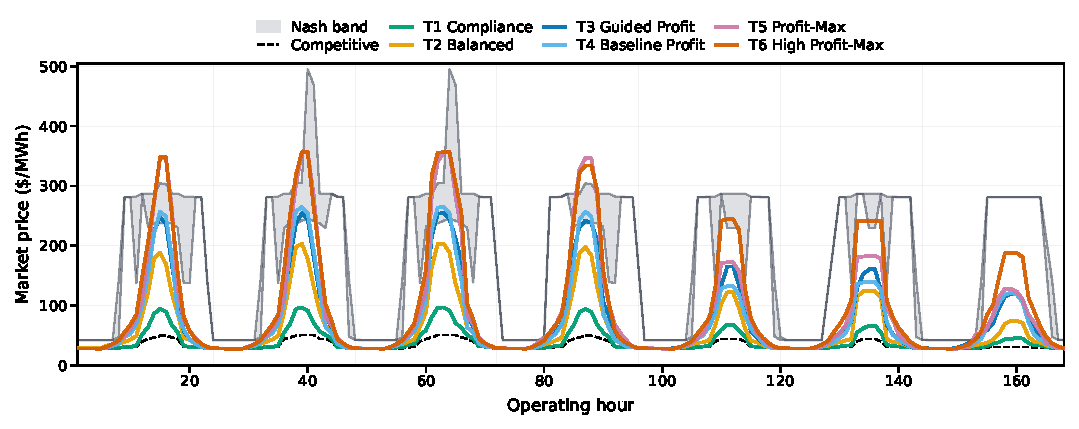
\includegraphics[
        width=0.90\textwidth,
        height=0.20\textheight,
        keepaspectratio
    ]{figures/figure_1_all_treatments_overlay_twocolumn}
    \caption{Hourly price trajectories by prompt treatment. Lines show treatment-average prices for all six prompt objectives; the dashed line shows the perfect competition benchmark and the shaded band shows the Nash benchmark range. More profit-oriented prompt treatments produce higher prices during peak and near-scarcity hours.}
    \label{fig:price_trajectories}
    \vspace{-0.6em}
\end{figure*}
% Table II: Treatment-level outcomes with vertically stacked confidence intervals
% Requires: \usepackage{booktabs}

\begin{table*}[t]
\centering
\caption{Treatment-Level Outcomes by Prompt Objective}
\label{tab:treatment_summary}
\scriptsize
\renewcommand{\arraystretch}{1.12}
\setlength{\tabcolsep}{3.6pt}
\begin{tabular}{@{}lrrrrr@{}}
\toprule
Treatment & Prompt $S_t$ & TARJ orient. & Mean markup & $\Delta P$ (\$/MWh) & $\Delta \Pi$ (\$M) \\
\midrule
T1 Compliance & $-0.134$ &
\begin{tabular}{@{}c@{}}$-0.011$\\{\scriptsize [$-0.015$, $-0.007$]}\end{tabular} &
\begin{tabular}{@{}c@{}}1.144\\{\scriptsize [1.129, 1.159]}\end{tabular} &
\begin{tabular}{@{}c@{}}6.87\\{\scriptsize [5.87, 7.90]}\end{tabular} &
\begin{tabular}{@{}c@{}}7.33\\{\scriptsize [6.31, 8.00]}\end{tabular} \\
\addlinespace[0.25em]
T2 Balanced & 0.009 &
\begin{tabular}{@{}c@{}}0.028\\{\scriptsize [0.024, 0.032]}\end{tabular} &
\begin{tabular}{@{}c@{}}1.591\\{\scriptsize [1.547, 1.632]}\end{tabular} &
\begin{tabular}{@{}c@{}}25.32\\{\scriptsize [21.98, 28.73]}\end{tabular} &
\begin{tabular}{@{}c@{}}26.77\\{\scriptsize [23.59, 29.72]}\end{tabular} \\
\addlinespace[0.25em]
T3 Guided Profit & 0.060 &
\begin{tabular}{@{}c@{}}0.057\\{\scriptsize [0.054, 0.060]}\end{tabular} &
\begin{tabular}{@{}c@{}}1.919\\{\scriptsize [1.848, 1.990]}\end{tabular} &
\begin{tabular}{@{}c@{}}40.67\\{\scriptsize [36.60, 44.89]}\end{tabular} &
\begin{tabular}{@{}c@{}}42.43\\{\scriptsize [38.12, 47.12]}\end{tabular} \\
\addlinespace[0.25em]
T4 Baseline Profit & 0.125 &
\begin{tabular}{@{}c@{}}0.066\\{\scriptsize [0.061, 0.070]}\end{tabular} &
\begin{tabular}{@{}c@{}}1.883\\{\scriptsize [1.769, 1.998]}\end{tabular} &
\begin{tabular}{@{}c@{}}38.26\\{\scriptsize [31.97, 44.57]}\end{tabular} &
\begin{tabular}{@{}c@{}}40.04\\{\scriptsize [28.20, 49.31]}\end{tabular} \\
\addlinespace[0.25em]
T5 Profit-Max & 0.132 &
\begin{tabular}{@{}c@{}}0.065\\{\scriptsize [0.061, 0.068]}\end{tabular} &
\begin{tabular}{@{}c@{}}2.382\\{\scriptsize [2.267, 2.523]}\end{tabular} &
\begin{tabular}{@{}c@{}}56.15\\{\scriptsize [49.11, 62.95]}\end{tabular} &
\begin{tabular}{@{}c@{}}58.85\\{\scriptsize [56.32, 61.41]}\end{tabular} \\
\addlinespace[0.25em]
T6 High Profit-Max & 0.147 &
\begin{tabular}{@{}c@{}}0.067\\{\scriptsize [0.064, 0.070]}\end{tabular} &
\begin{tabular}{@{}c@{}}2.700\\{\scriptsize [2.593, 2.809]}\end{tabular} &
\begin{tabular}{@{}c@{}}65.30\\{\scriptsize [60.12, 70.63]}\end{tabular} &
\begin{tabular}{@{}c@{}}68.15\\{\scriptsize [61.41, 74.89]}\end{tabular} \\
\bottomrule
\end{tabular}

\vspace{1.0em}
\begin{minipage}{0.90\textwidth}
\footnotesize
\emph{Note:} Bracketed values report 95\% bootstrap intervals. $S_t$ is the SBERT prompt profit-minus-compliance orientation. $\Delta P$ is average price increase relative to the competitive benchmark, and $\Delta \Pi$ is firm profit gain. Price, markup, and TARJ intervals resample seed--day blocks within treatment; firm-profit intervals resample seed-level treatment runs. TARJ orientation is post-treatment and is reported as behavioral alignment rather than a causal mechanism.
\end{minipage}
\vspace{-0.4em}
\end{table*} 

\subsection{Economic Benchmark Comparison}

We first compare LLM-agent market outcomes with the perfect competition and strategic Nash Equilibrium benchmarks. The perfect competition benchmark clears the same market using cost-based offers, so it provides the reference price path for measuring price impacts. The Nash benchmark provides a useful strategic reference because it represents equilibrium behavior under the same market environment and markup grid available to the LLM agents. Since some hours have multiple pure-strategy equilibria, we report an hourly Nash price band rather than a single price. The band is not evidence that the agents solved for equilibrium. Instead, it shows whether their bids move market outcomes away from the perfect competition benchmark and toward the strategically elevated prices that are feasible under model conditions.

Figure~\ref{fig:price_trajectories} shows that the prompt treatments produce visibly different price trajectories. As the profit orientation ($S_t$) of treatments increases, we observe more aggressive bidding behavior and higher market prices.  T1 Compliance remains closest to the perfect competition benchmark. Intermediate treatments raise prices during high-load hours, while the most profit-oriented treatments, especially T5 Profit-Max and T6 High Profit-Max, move prices closer to strategic pricing and the Nash band during peak and near-scarcity periods. This is consistent with the electricity-market intuition that strategic markups matter most when supply is tight and the marginal unit has greater price-setting influence.


\subsection{Treatment-Level Outcomes}

Table~\ref{tab:treatment_summary} summarizes the treatment-level semantic and market outcomes. As objectives become more profit-oriented, average price impacts generally increase: from $\$6.87$/MWh under T1 Compliance to $\$65.30$/MWh under T6 High Profit-Max. The ordering is not perfectly monotonic, since T3 has lower prompt orientation than T4 but a slightly higher average price impact. Nevertheless, there is a clear emerging pattern. Compliance-oriented prompting produces outcomes closest to the perfect competition benchmark, while increasingly profit-oriented prompting pushes prices upward toward the strategic price range indicated by the Nash band.

The markup and profit results show the same directional pattern. Mean markup increases from 1.144 under T1 to 2.700 under T6, and firm profit gain rises from \$7.33M to \$68.15M. These increases suggest that more aggressive profit-maximizing language pushes agents to submit higher markups and capture larger profits. However, this effect is bounded. In this case study, prices are limited by the finite markup grid, the underlying supply stack, demand conditions, and the availability of the backstop resource. The Nash band therefore provides a useful reference for interpreting the upper strategic range. It does not represent a hard cap on every possible non-equilibrium bid outcome, but it shows the elevated price region consistent with equilibrium play under the same model assumptions. The main result is that changing only the objective block of the prompt moves simulated bidding behavior from near-competitive outcomes toward this strategic benchmark range.


\subsection{Semantic Orientation, Prompt Selection, and Market Outcomes}

Figure~\ref{fig:semantic_orientation} relates semantic profit-minus-compliance orientation to market outcomes, showing whether the SBERT ordering used to characterize and select prompts is reflected in bidding behavior. Panels A and B use the SBERT orientation of the objective prompt, which is measured before simulation and represents the treatment's position along the compliance-profit axis. Panels C and D use the SBERT orientation of generated TARJ rationales, which are post-treatment text artifacts produced by the agents during the simulation. Prompt orientation therefore measures the intervention, while TARJ orientation measures agent-generated explanations for bidding behavior.
\begin{figure}[!t]
    \centering
    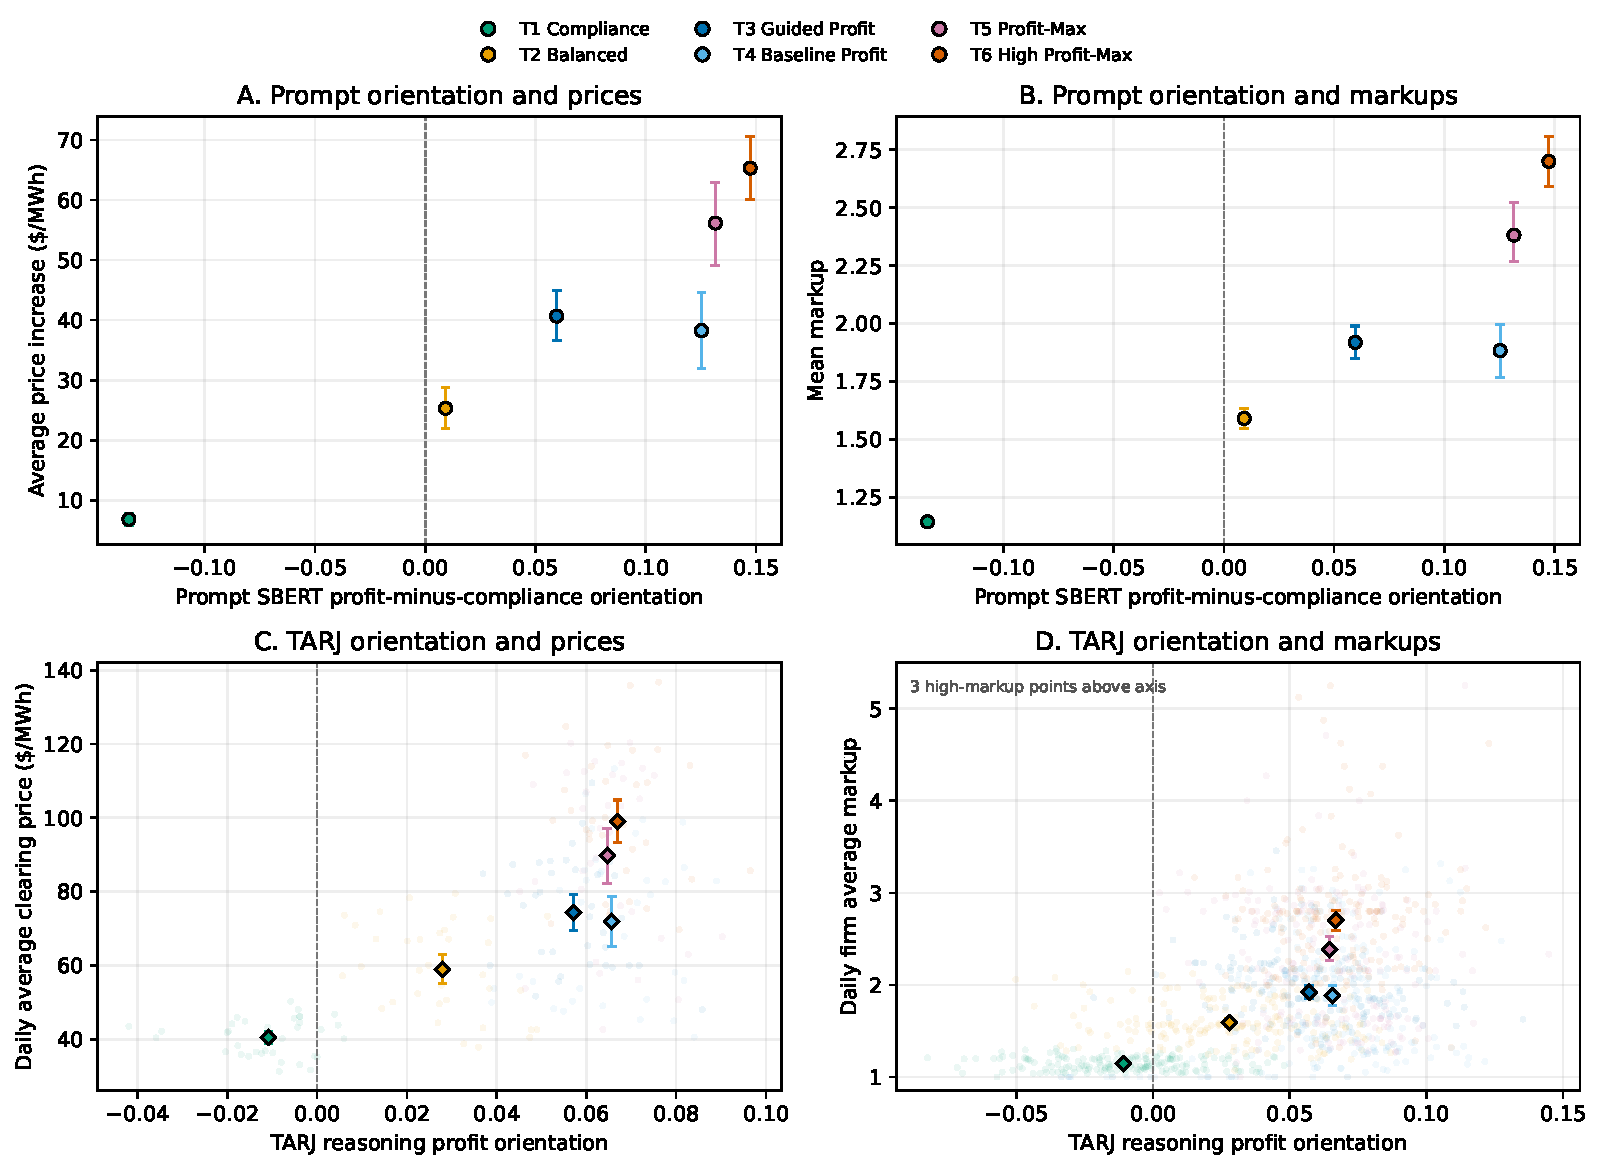
\includegraphics[
        width=0.99\columnwidth,
        height=0.55\textheight,
        keepaspectratio
    ]{figures/figure_2_semantic_orientation_main_no_spearman}
    \caption{Semantic orientation, prices, and bidding behavior. Panels A--B compare prompt orientation with average price increases and mean markups; Panels C--D compare TARJ orientation with daily prices and firm markups. Error bars report 95\% bootstrap intervals.}
    \label{fig:semantic_orientation}
    \vspace{-0.8em}
\end{figure}
The main statistical result is a treatment-level relationship between prompt orientation and market outcomes, estimated using \eqref{eq:dose_response}.

\begin{table}[!t]
\centering
\caption{SBERT Orientation Regression Coefficients}
\label{tab:dose_response_summary}
\scriptsize
\renewcommand{\arraystretch}{1.05}
\setlength{\tabcolsep}{2.8pt}
\begin{tabular}{@{}lcccc@{}}
\toprule
Outcome & $\hat{\beta}_{0.1}$ & 95\% CI & $R^2$ & $p$ \\
\midrule
$\Delta P$ (\$/MWh) & 18.17 & [7.85, 28.49] & 0.857 & 0.008 \\
Mean markup & 0.465 & [0.153, 0.778] & 0.810 & 0.014 \\
Firm profit (\$M) & 18.93 & [8.21, 29.65] & 0.857 & 0.008 \\
Consumer payments (\$M) & 19.02 & [8.35, 29.70] & 0.860 & 0.008 \\
Mean TARJ orientation & 0.029 & [0.021, 0.036] & 0.967 & $<0.001$ \\
\bottomrule
\end{tabular}

\vspace{0.25em}
\begin{minipage}{0.96\columnwidth}
\footnotesize
\emph{Note:} Estimates come from treatment-level regressions $\bar{Y}_t=\alpha+\beta S_t+\epsilon_t$, where $S_t$ is prompt SBERT profit-minus-compliance orientation. Coefficients are scaled to a 0.1 increase in prompt orientation. CIs use OLS standard errors across the six treatment means with four residual degrees of freedom.
\end{minipage}
\vspace{-0.8em}
\end{table}

As shown in Table~\ref{tab:dose_response_summary}, a 0.1 increase in prompt orientation is associated with an estimated $\$18.17$/MWh increase in average price impact relative to the perfect competition benchmark. The same pattern appears for bidding aggressiveness: a 0.1 increase in prompt orientation is associated with a 0.465 increase in mean markup. The table also shows positive associations with firm profit gains, consumer payment increases, and TARJ reasoning orientation. These relationships are also statistically strong within the six-treatment design, with the $R^2$ values in Table~\ref{tab:dose_response_summary} ranging from 0.810 to 0.967, and all reported $p$-values are below 0.05. Because the regressions use treatment-level means, we interpret these statistics as evidence of within-case alignment rather than as broad population-level inference.

A similar relationship also appears in distributional market outcomes. A 0.1 increase in prompt orientation is associated with an estimated $\$18.93$M increase in firm profit gain and a $\$19.02$M increase in consumer payments. Prompt orientation is also strongly associated with generated reasoning language. A 0.1 increase in prompt orientation is associated with a 0.029 increase in mean TARJ reasoning orientation. This is the expected direction under the proposed framework. Prompts that are semantically closer to profit maximization are intended to induce more aggressive bidding, higher market prices, and higher firm profits if the prompt intervention is functioning properly.

The TARJ-orientation panels (C and D) provide a secondary result. More profit-oriented generated reasoning accompanies higher prices and more aggressive markups, but this relationship is interpreted differently from the prompt-orientation relationship. TARJ text is generated after the prompt intervention, so it is treated as a way to analyze agent reasoning in addition to bidding behavior. This alignment is important because it suggests that the framework is not only detecting changes in bidding behavior, but also validating that prompt meaning, generated reasoning, and bidding posture are aligned.


\section{Discussion}
The results support a focused methodological conclusion: prompt objectives can be treated as controlled interventions, and SBERT orientation provides an interpretable measure for ordering, selecting, and evaluating their semantic direction. Holding the market environment, action space, prompt structure, and model configuration fixed, more profit-oriented objective blocks generally produce higher markups, prices, and firm profits.

Competitive market and Nash band benchmarks anchor this semantic result in economic terms. Figure~\ref{fig:price_trajectories} shows that price elevation is concentrated in peak and near-scarcity hours, where strategic markups have the greatest opportunity to affect clearing prices. The perfect competition benchmark provides the cost-based reference path, while the Nash band provides an equilibrium reference point under the finite markup grid. As prompts become more profit-oriented, agent bids move market outcomes away from the perfect competition benchmark and closer to the Nash benchmark band. This does not mean that the agents solved for or converged to Nash equilibrium. Rather, it shows that profit-oriented objectives induce more aggressive bidding behavior that moves outcomes closer to the highest-profit strategic benchmark available in the simplified action space.

The SBERT orientation regression coefficients provide quantitative evidence for this trend. A 0.1 increase in prompt orientation is associated with higher price impacts, markups, firm profit gains, and consumer payment increases. These estimates are useful because they quantify the relationship between prompt orientation and economic units. These estimates should be interpreted as descriptive evidence from a controlled case study rather than as large-sample statistical inference. The relationship is estimated from six treatment-level observations, so the result is informative about the prompt interventions studied here but not yet sufficient to establish a general law across all possible prompt treatments.

The semantic results also show that prompt orientation and generated reasoning orientation move in the same direction. Both are aligned with the agents' bidding posture. We find that more profit-oriented objectives produce higher markups and prices, and more profit-oriented TARJ language accompanies more aggressive bidding behavior. This supports the use of semantic orientation not only as a prompt-design measure, but also as a diagnostic for whether the agent's generated reasoning artifacts are directionally consistent with its actions.



\section{Conclusion}

This paper introduces a semantic-orientation framework for selecting, designing, and evaluating LLM bidding-agent objectives in a stylized electricity-market simulation. The experiment varies only the objective block of a modular prompt while holding the market environment, information set, response format, action space, model configuration, and TARJ structure fixed. SBERT is used to measure the semantic direction of that intervention along a profit-versus-compliance axis.

The main contribution of this paper is a framework for using prompt objectives as controlled interventions and semantic-orientation analysis as a way to evaluate their influence on LLM-agent behavior. In the simulated market, more profit-oriented prompting leads to higher markups and prices relative to the perfect competition benchmark, especially during peak and near-scarcity hours. SBERT orientation regressions support the same directional pattern. Generated TARJ reasoning orientation also moves with bidding posture. Table~\ref{tab:dose_response_summary} shows that a 0.1 increase in prompt orientation is associated with a 0.029 increase in mean TARJ reasoning orientation, with $R^2=0.967$ and $p<0.001$. This suggests that semantic analysis can help verify whether prompt meaning, agent-generated reasoning, and submitted bids are directionally aligned.

Future work can proceed in several directions. Our framework can be tested in more realistic power-market environments with richer operational constraints, firm portfolios, uncertainty, storage, renewable generation, and repeated market interaction. Future studies can also formalize the evaluation framework and test its robustness across additional LLM models, embedding methods, prompt grids, and market designs. Together, these extensions would clarify how general the observed prompt-orientation effects are and how semantic measurement can be used to systematically evaluate LLM-agent behavior in electricity-market settings.


\section*{Disclaimer}

The views expressed in this paper are those of the authors and do not reflect the views of PJM Interconnection, L.L.C. or its Board of Managers, of which Le Xie is a member.

% ------------------------------------------------------------------
% References
% ------------------------------------------------------------------

\bibliographystyle{IEEEtran}
\bibliography{references}

\end{document}